% ---------------------------------------------------------------------------
% Supplementary Figures (separate submission item)
%
% The target journal requires supplementary material to be uploaded as a file
% of its own, so the three supplementary figures live here instead of at the
% end of manuscript.tex. Figure numbering (S1-S3) matches the citations in the
% main text, which refer to them by hard-coded label.
%
% The page geometry reproduces the published text block of the journal (174.9 mm
% wide, measured on a published article) rather than the narrower author
% template, so that a figure placed at \textwidth prints at the size it was
% drawn at and the type inside it keeps the point size declared in its
% generating script.
% ---------------------------------------------------------------------------
\documentclass[11pt]{article}

\usepackage[T1]{fontenc}
\usepackage[utf8]{inputenc}
\usepackage{newtxtext}
\usepackage{amsmath,amssymb}
\usepackage{graphicx}
\usepackage[
  paperwidth=210mm,
  paperheight=279mm,
  left=17.55mm,
  right=17.55mm,
  top=22mm,
  bottom=22mm,
]{geometry}
\usepackage[hidelinks]{hyperref}

\setlength{\parindent}{0pt}

\begin{document}

% The journal asks every supplementary file to carry the article title, the journal name, the
% author and the affiliation and e-mail address of the corresponding author.
\begin{center}
{\large\bfseries Supplementary Figures}\\[2.5mm]
{\normalsize Edge-level causal graph comparison across 33 TCGA cohorts reveals tissue-specific regulatory structure and prognostic hub genes}\\[1.5mm]
{\small Functional \& Integrative Genomics}\\[1.5mm]
{\small Shuaidong Gao}\\[0.8mm]
{\small Chongqing Institute of Foreign Studies, Qijiang Campus, Chongqing 401420, China}\\[0.8mm]
{\small Corresponding author: gaoshuaidong@stu.cqifs.edu.cn}
\end{center}

\vspace{5mm}

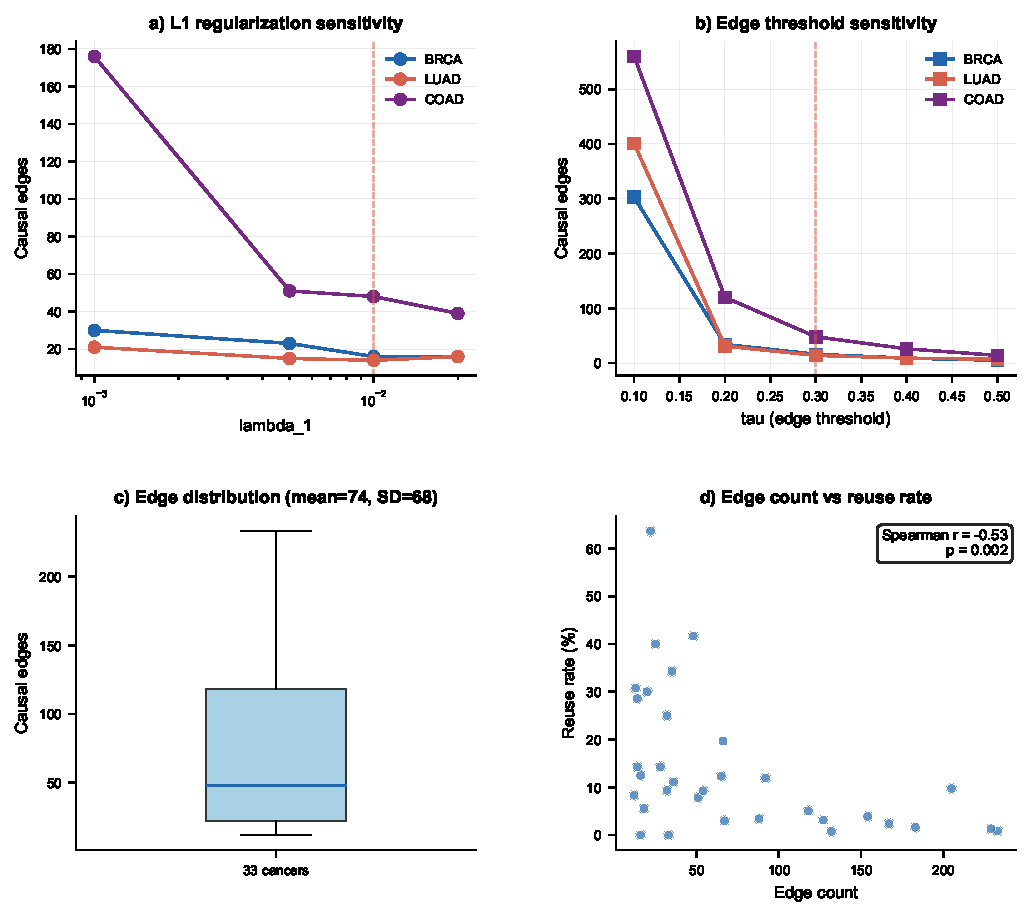
\includegraphics[width=\textwidth]{figures/fig4_sensitivity.pdf}

\vspace{2.5mm}
{\small\textbf{Fig.~S1} Parameter sensitivity of the NOTEARS pipeline. \textbf{a)} $\ell_1$ regularization sensitivity for three representative cancers; $\lambda_1 = 0.01$ selected (dashed). \textbf{b)} Edge threshold $\tau$ sensitivity; $\tau = 0.3$ selected (dashed). \textbf{c)} Edge count distribution across 33 cancers (boxplot; mean 74.1, SD 67.7). \textbf{d)} Edge count vs per-cancer reuse rate (Spearman $r = -0.53$, $p = 0.002$)}

\clearpage

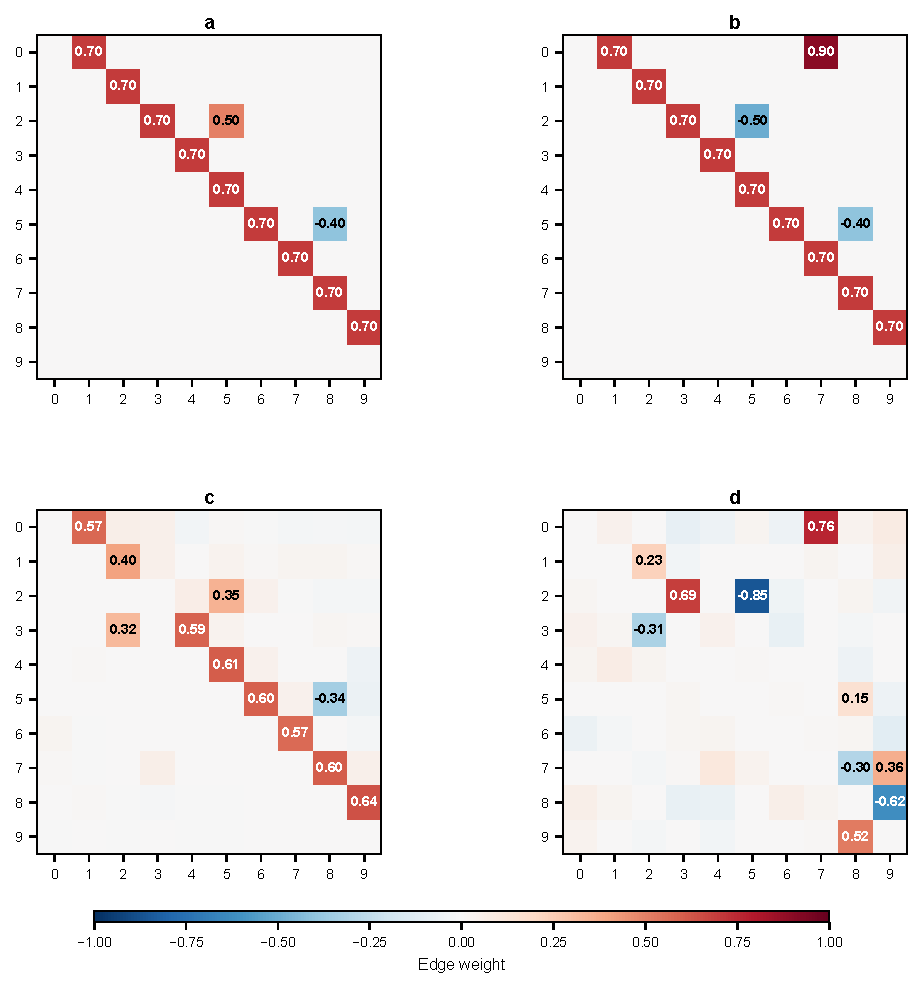
\includegraphics[width=\textwidth]{figures/fig1_synthetic.pdf}

\vspace{2.5mm}
{\small\textbf{Fig.~S2} Two-stage decomposition validation on a synthetic Erd\H{o}s--R\'enyi DAG ($d=10$, $K=3$). \textbf{a)} Ground truth shared backbone $W_0$ (11 edges). \textbf{b)} Ground truth Batch~1: rewired edge $2\to5$ (sign-flipped) and new edge $0\to7$. \textbf{c)} Recovered $\hat{W}_0$ from Stage~2 DAG projection (10/11 shared edges above $\tau=0.2$, $h(W_0)=5.21\times10^{-6}$). \textbf{d)} Deviation matrix $\Delta_1=\hat{W}_1-\hat{W}_0$ for the rewired batch. Overall recall: 14/15 ground-truth edges recovered ($=0.93$); see Table~2 of the main text for Precision, F1, FDR, and SHD}

\clearpage

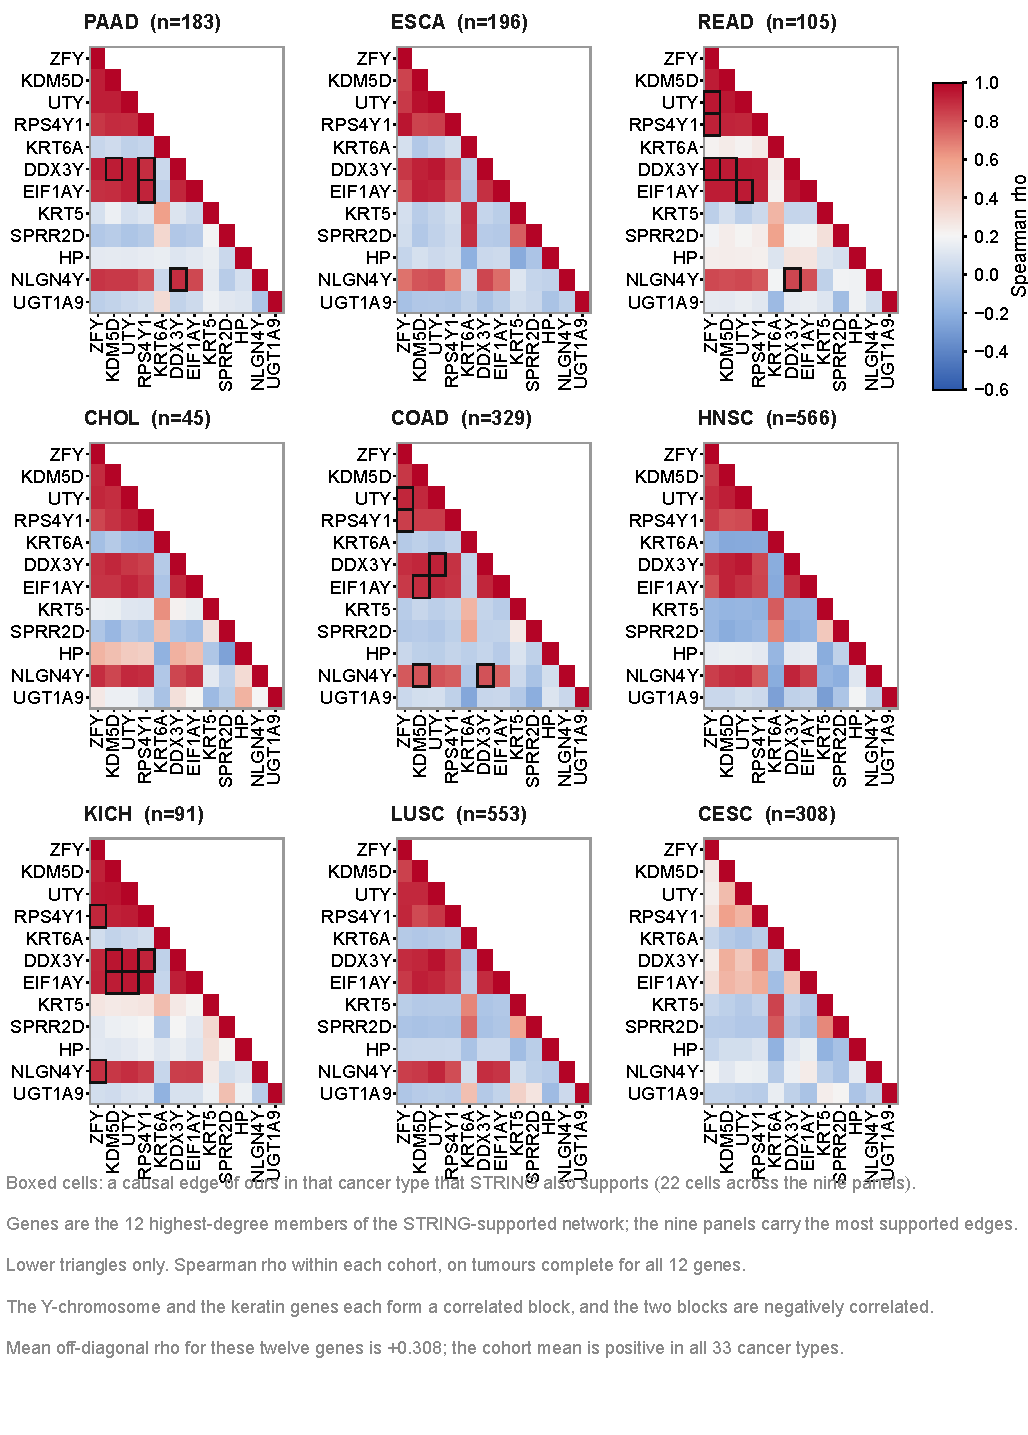
\includegraphics[width=0.82\textwidth]{figures/fig_corr.pdf}

\vspace{2.5mm}
{\small\textbf{Fig.~S3} Co-expression structure of the supported network. Lower triangles of the Spearman correlation matrix of the twelve highest-degree genes of the STRING-supported network, computed within each of the nine cohorts carrying the most supported edges. Boxed cells mark a causal edge of ours that STRING also supports. The Y-chromosome genes and the keratin genes each form a correlated block, and the two blocks are negatively correlated}

\clearpage

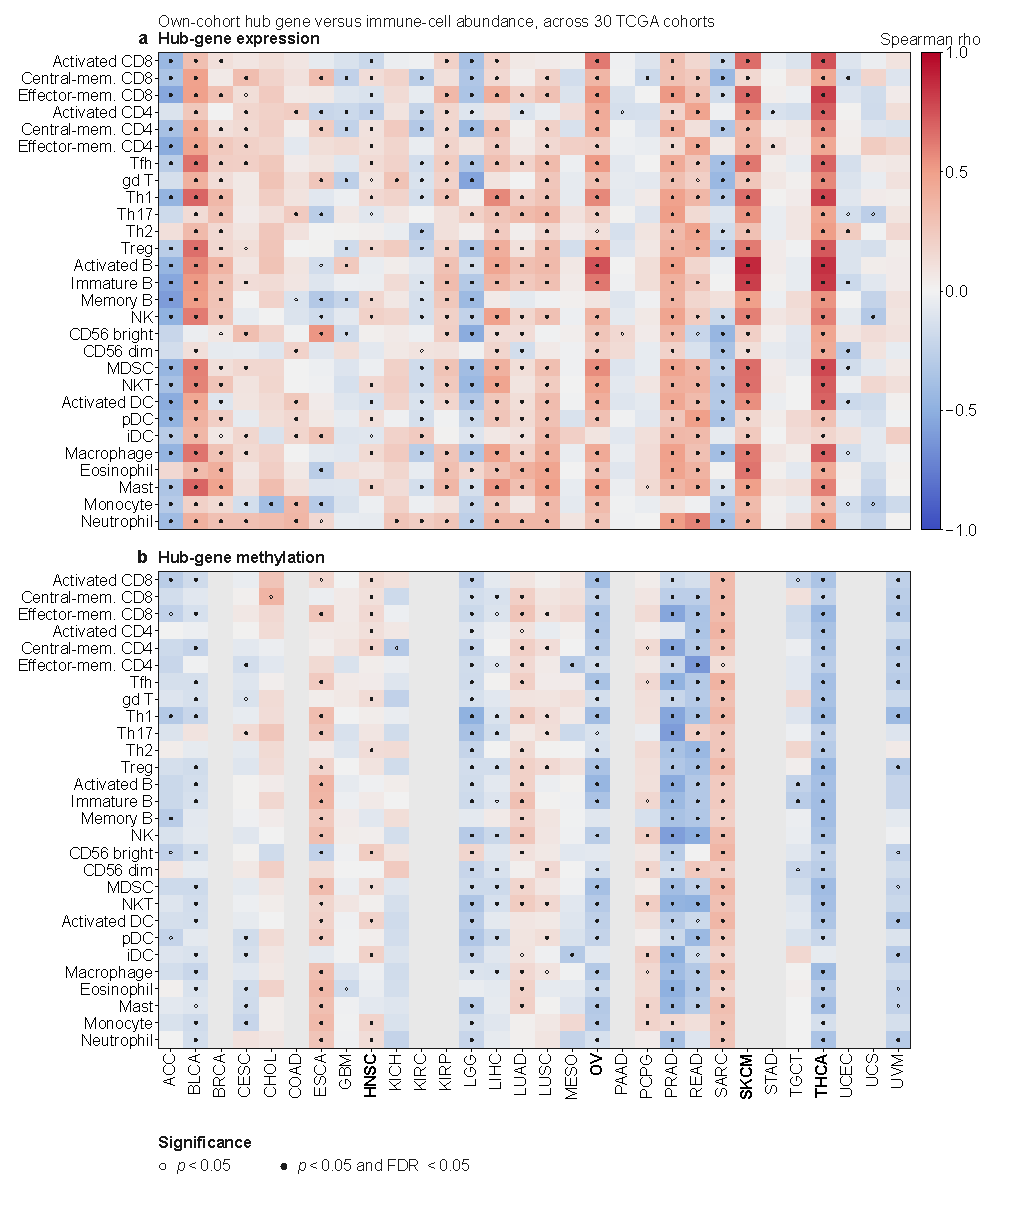
\includegraphics[width=0.92\textwidth]{figures/fig_immune.pdf}

\vspace{2.5mm}
{\small\textbf{Fig.~S4} Immune-microenvironment association of each cohort's own hub gene. \textbf{a)} Hub-gene expression and \textbf{b)} hub-gene methylation against the abundance of the 28 TISIDB immune cell types, for the 30 cohorts carrying an immune profile; each cell is the Spearman $\rho$ between that cohort's own hub gene and that cell type, with significance marked as in the legend. Bold cohort labels mark hubs that are themselves immune-lineage markers; gray columns carry no data, methylation covering 21 cohorts. Expression is predominantly positive (306 of the 416 significant pairs) and methylation predominantly negative (175 of 270); the copy-number layer, with only 44 of 756 pairs significant, is not drawn. Excluding the four immune-lineage hubs, the hub still exceeds the other genes of its own network in 57.7\% of 728 pairs ($p = 4.4 \times 10^{-12}$), a modest effect (median $|\rho|$ 0.145 versus 0.122) that reverses in 10 of 26 cohorts}

\end{document}
